\documentclass[12pt]{amsart}
\usepackage{latexsym}
\usepackage{amssymb,amsmath}
\usepackage[pdftex]{graphicx}
\usepackage{enumerate}
\usepackage{endnotes}
%\usepackage{extpfeil}
\usepackage{hyperref}
\usepackage[usenames,dvipsnames]{xcolor}
\usepackage{stackrel}
\usepackage{bbm}
\usepackage{tikz}
\usepackage[margin=1in]{geometry}
\usepackage{hyperref}
\usepackage{listings}
\usepackage{courier}
\usepackage{color}
\usepackage{upgreek}

\lstset{
	basicstyle=\small\ttfamily,
	keywordstyle=\color{blue},
	language=python,
	xleftmargin=16pt,
}

\usetikzlibrary{arrows,chains,matrix,positioning,scopes}

\makeatletter
\tikzset{join/.code=\tikzset{after node path={%
\ifx\tikzchainprevious\pgfutil@empty\else(\tikzchainprevious)%
edge[every join]#1(\tikzchaincurrent)\fi}}}
\makeatother
%
\tikzset{>=stealth',every on chain/.append style={join},
         every join/.style={->}}
\tikzstyle{labeled}=[execute at begin node=$\scriptstyle,
   execute at end node=$]
\usetikzlibrary{patterns}

\usetikzlibrary{decorations.pathreplacing}

\DeclareSymbolFont{bbold}{U}{bbold}{m}{n}
\DeclareSymbolFontAlphabet{\mathbbold}{bbold}

\newtheorem{thm}{Theorem}[section]
\newtheorem{ithm}{Theorem}
\newtheorem{lem}[thm]{Lemma}
\newtheorem{conj}[thm]{Conjecture}
\newtheorem{prop}[thm]{Proposition}
\newtheorem{cor}[thm]{Corollary}

\theoremstyle{definition}
\newtheorem{defi}[thm]{Definition}
\newtheorem{example}[thm]{Example}
\newtheorem{exercise}[thm]{Exercise}
\newtheorem{rem}[thm]{Remark}


   
\def\B{{\mathbb B}}
\def\C{{\mathbb C}}
\def\D{{\mathbb D}}
\def\Fp{{\mathbb F}_p}
\def\Fell{{\mathbb F}_{\ell}}
\def\F{{\mathbb F}}
%\def\H{{\mathbb H}}
\def\M{{\mathbb M}}
\def\N{{\mathcal N}}
\def\O{{\mathcal O}}
\def\0{{\mathbb 0}}
\def\P{{{\mathbb P}}}
\def\Q{{\mathbb Q}}
\def\R{{\mathbb R}}
\def\T{{\mathbb T}}
\def\Z{{\mathbb Z}}

\newcommand{\sol}{_{a^p,b^p,c^p}}
\newcommand{\bound}{\partial}
\newcommand{\la}[1]{\mathfrak{#1}}
\newcommand{\im}{\text{im} \hspace{0.1em} }
\newcommand{\ann}{\text{Ann} \hspace{0.1em} }
\newcommand{\rank}{\text{rank} \hspace{0.1em} }
\newcommand{\coker}[1]{\text{coker}\hspace{0.1em}{#1}}
\newcommand{\sgn}{\text{sgn}}
\newcommand{\lcm}{\text{lcm}}
\newcommand{\re}{\text{Re}  \hspace{0.1em} }
\newcommand{\ext}[1]{\text{Ext}(#1)}
\newcommand{\Hom}[1]{\text{Hom}(#1)}
\newcommand{\End}[1]{\text{End(#1)}}
\newcommand{\bs}{\setminus}
\newcommand{\rpp}[1]{\mathbb{R}\text{P}^{#1}}
\newcommand{\cpp}[1]{\mathbb{C}\text{P}^{#1}}
\newcommand{\tr}{\text{tr}\hspace{0.1em} }
\newcommand{\inner}[1]{\langle {#1}\rangle}
\newcommand{\tensor}{\otimes}
\newcommand{\Cl}{\text{Cl}}
\renewcommand{\sp}[1]{\text{Sp}_{#1}}
\newcommand{\GL}{\text{GL}}
\newcommand{\PGL}{\text{PGL}}
\renewcommand{\sl}[1]{\text{SL}_{#1}}
\newcommand{\so}[1]{\text{SO}_{#1}}
\newcommand{\SO}{\text{SO}}
\newcommand{\pso}[1]{\text{PSO}_{#1}}
\renewcommand{\o}[1]{\text{O}_{#1}}
\renewcommand{\sp}[1]{\text{Sp}_{#1}}
\newcommand{\psp}[1]{\text{PSp}_{#1}}
\newcommand{\Span}{\rm Span}
\newcommand{\Frob}{\rm Frob}
\newcommand{\tor}{\rm tor}
\newcommand{\rad}{{\rm{rad}}}
\newcommand{\denom}{\rm denom}
\renewcommand{\bar}{\overline}
\newcommand{\notdiv}{\nmid}
\newcommand{\pfrac}[2]{\left( \frac{#1}{#2} \right)}
\newcommand{\bfrac}[2]{\left| \frac{#1}{#2} \right|}
\newcommand{\Ell}{\rm{Ell}}
\newcommand{\AV}{\rm{AV}}
\newcommand{\Gal}{\text{Gal}}
\newcommand{\ord}{{\rm{ord}}}

\newcommand{\kron}[2]{\bigl(\frac{#1}{#2}\bigr)}
\newcommand{\leg}[2]{\Biggl(\frac{#1}{#2}\Biggr)}

\DeclareSymbolFont{bbold}{U}{bbold}{m}{n}
\DeclareSymbolFontAlphabet{\mathbbold}{bbold}

%%%%%%%%%%%%%% COLOR COMMENTS! %%%%%%%%%%%%%%%
\usepackage{color}
\newcommand{\david}[1]{{\color{blue} \sf $\spadesuit\spadesuit\spadesuit$ David: [#1]}}
\newcommand{\bjorn}[1]{{\color{red} \sf $\clubsuit\clubsuit\clubsuit$ Bjorn: [#1]}}

% changed above definition to make comments disappear
%\newcommand{\david}[1]{}
%\newcommand{\bjorn}[1]{}


\begin{document}

\title{Perfect Powers in Lucas Sequences via Galois Representations}
\author{Jesse Silliman and Isabel Vogt}

\maketitle


\section{Introduction}
The Fibonacci Sequence, perhaps the simplest linear recurrence sequence, begins as \[\underline{0},\underline{1},\underline{1},2,3,5,\underline{8},13,21,34,55,89,\underline{144},233, \cdots\] The reader will no doubt note that the underlined terms are perfect powers. Although a folklore conjecture for many years, a proof that these underlined terms are in fact the \emph{only} perfect powers in the Fibonacci sequence remained decidedly elusive via classical methods. Various partial results in this direction, based mainly on elementary congruences and Baker's theory of linear forms in logarithms, ruled out specific $p$th powers for small primes $p$. In 2006, this conjecture was finally proven in an impressive paper of Bugeaud, Mignotte, and Siksek \cite{siksek06}. In contrast with previous results, the proof relied upon what has come to be termed the ``modular method", connecting the Diophantine behavior of the Fibonacci sequence to the arithmetic properties of elliptic curves.

Here, we revisit this strategy with two aims. First, we would like to apply the modular method to find all perfect powers in other examples of linear binary recurrence relations.  In particular, we study natural generalizations of the Fibonacci sequence known as Lucas sequences.  A Lucas sequence is a nondegenerate recurrence sequence defined by \[ u_n = b u_{n-1} + c u_{n-2}, \qquad u_0 = 0, u_1 = 1, \] for $b$ and $c$ nonzero integers.  The Diophantine problem of interest, of course, is to study integer solutions $(n,y,p)$, $n > 0$, $p$ prime, to \begin{equation}\label{the_eqn}u_n = y^p.\end{equation}
Solutions of the form $0=0^p$ or $1 = 1^p$ are called trivial, as they are perfect $p$th powers for any $p$. 

We develop an effective method, whose correctness is conditional on the Frey-Mazur Conjecture (see \ref{FreyMazur}), to determine all of the perfect powers in a Lucas sequence with $b$ and $c$ relatively prime.  We use this method in Section \ref{examples} to prove the following theorem:

\begin{ithm}\label{cond_ex}
Assume the Frey-Mazur Conjecture.  For $(b,c)$ a nondegenerate Lucas sequence with $1 \leq b,c \leq 10$ relative prime, the only perfect powers occur for $p \leq 19$.
%besides $u_0=0,u_1=1$, and $u_2 = b$ (in the cases $b$ is a perfect power) occur for $n \leq 7$.
\end{ithm}

***need to get the bound on $n$ in terms of $p$, then we think we can prove the stronger theorem on all of the perfect powers***

%The exact perfect powers are given in \ref{cond_ex_inplace}.  

In some cases, our methods do not require the Frey-Mazur Conjecture.  Namely, we prove the following theorem:

\begin{ithm}\label{explicit_eg_thm}
For the following values of $b$ and $c$:
\begin{equation}\label{examples} (b,c) = (3,-2), (5,-6), (7,-12), (17,-72), (9,-20) \end{equation}
the Lucas sequence $u_n$ has no nontrivial $p$th powers, except $u_2 = 3^2$ in $(9,-20)$.  Further these are the only sequences with $b^2+4c = 1$ that map to levels $N$ such that $\dim S_2(\Gamma_0(N)) = 0$.
\end{ithm}

Note that for $(b,c) = (3,-2)$, this provides an alternative proof to the theorem that there are no perfect powers in the Mersenne numbers $2^n - 1$.  This is a specific case of Catalan's Conjecture on perfect powers differing by $1$, recently proven by Mihaelescu \cite{mih04}.  These specific unconditional examples, as well as the necessary classical and modular techniques, are covered in Sections \ref{classicalresults} and \ref{mod_method}.

The modular method is highly effective for the Diophantine problems encountered in Theorem \ref{explicit_eg_thm} as there are no weight 2 newforms for the levels of interest, allowing a contradiction similar to that in Fermat's Last Theorem.  However, there are only finitely many levels $N$ for which the space of cuspforms is empty; in fact this implies $N \leq 60$.  The number of newforms of level $N$ grows roughly linearly, thus as $N$ increases, more clever techniques are necessary in order to show that the newforms of a given level cannot correspond to nontrivial solutions to the Diophantine problem.  This usually involves exploiting congruence conditions placed on Fourier coefficients or the existence of complex multiplication, as in \cite{bennett04}.  If a solution could exist, one might proceed as in \cite{siksek06}, deriving ``local conditions" on the index of the solution, which can then be combined with classical methods.  None of these techniques, though, work in general, and often rely heavily on details of the problem at hand, sometimes combined with nontrivial amounts of computation.


This leads us to the second goal of our paper, which is to use modular methods combined with the powerful Frey-Mazur Conjecture to obtain general results about perfect powers in Lucas sequences. It was shown independently by Petho \cite{petho82} and Shorey and Stewart \cite{shorey83} that there are only finitely many perfect powers in any linear recurrence sequence.  Although their proofs implied the bound could be made effective, an \emph{explicit} effective bound on $p$ has not been published to the knowledge of the authors.  In section \ref{genthmproof}, we answer this question by proving the following result conditional on the Frey-Mazur Conjecture.


\begin{ithm}\label{condbound}
Assume the Frey-Mazur conjecture.  Let 
\[ \psi(N) = N \cdot \prod_{p|N} \left( 1 + \frac{1}{p} \right)\]
be the Dedekind $\psi$ function.  Consider a solution (n,y,p) to \eqref{the_eqn}, with $n > 6$ and $b,c$ relatively prime. Let $N = 2^8 \cdot \rad(c(b^2+4c))$. Then 
\[ p \leq \max\left\{17,   \psi(N)^{(\psi(N)/12+1)}, 3\log{|\alpha|} \cdot ( N+1)  \right\} \]
for $\alpha$ the dominant root of the characteristic polynomial $g(z) = z^2 -bz-c$.
\end{ithm}
This Theorem allows the conditional results covered in Section \ref{examples}.

\section{Classical Facts about Lucas Sequences}\label{classicalresults}


Let $(b,c) \in \Z \times \Z$ define the integral linear binary recurrence relation
\[ U_{n+2} = b\cdot U_{n+1}+ c\cdot U_n, \]
with characteristic polynomial and roots
\[ g(z) = z^2 - bz - c, \qquad \qquad \alpha, \beta = \frac{b \pm \sqrt{b^2+4c}}{2}.\]
The sequence is nondegenerate if $\alpha/\beta$ is not a root of unity.  Throughout this paper, we will refer to nondegenerate integral linear binary recurrence sequences as simply binary recurrence sequences.  In particular, let $u_n$ and $v_n$ denote the companion sequences specified by starting conditions
\[ u_0 = 0, u_1 = 1 \qquad \qquad v_0 = 2, v_1 = b .\]
The sequence $u_n$ is termed a Lucas sequence, and will be our main focus.  The $n$th terms of these sequences are given by 
\begin{equation}\label{binetform} u_n = \frac{\alpha^n - \beta^n}{\alpha - \beta} \qquad \qquad v_n = \alpha^n +\beta^n. \end{equation}
This formula easily implies the following two key facts
\begin{equation}\label{fib2} u_{2k} = u_kv_k \end{equation}
\begin{equation}\label{gen_diophan}(\alpha - \beta)^2u_n^2 = v_n^2 - 4(\alpha\beta)^n. \end{equation}
Both equations \ref{binetform} and \ref{gen_diophan} translate the question of perfect powers in recurrence sequences into a clear Diophantine context that will be the focus of the remaining sections of the paper.

\section{Some Immediate Results}

We begin a survey of some classes of recurrence sequences that can be dealt with immediately as one or both of their associated Diophantine equations \ref{binetform} and \ref{gen_diophan} have already been investigated.

\subsection{Pell Sequences with $b$ even and $c = -1$}

In this case, equation \ref{gen_diophan} reduces to
\[ (b^2-4)y^{2p}+4 = v_n^2, \]
and as $b^2-4 \equiv 0 \pmod{4}$, this gives an integral solution to 
\begin{equation}\label{pell} x^2 - Dy^{2p} = 1.\end{equation}
Bennett has studied these equations in \cite{bennett05} and proven the following general theorem
\begin{thm}
For $p \geq 3$ and $D$ not a square, and $x,y$ satisfying \ref{pell}, either $D = 2^{2p-2}a^{2p}-1, y = 2a$ or $p < (2e\cdot \rad(D))^{2\rad(D)^3}$.
\end{thm}
In addition, the paper finds all solutions to \ref{pell} for $D< 100$.  The proof of this theorem also relies upon the modular method.  Note that assuming the Frey-Mazur conjecture, our Theorem \ref{condbound} provides a stronger bound for sequences of this form.  In addition, Bennett found all solutions for $D< 100$.

\subsection{Sequences with $\beta = 1$}

Similarly when the smaller root $\beta=1$, the Diophantine equation \ref{gen_diophan} reduces to 
\[ \frac{\alpha^n - 1}{\alpha - 1} = y^p \]
which is a Nagell-Ljunggren equation.  This equation has been shown to have no nontrivial solutions for all values of $-10^4 \leq \alpha \leq 10^6$.  These sequences with $\beta = 1$ are those for which $b \geq 3$, $c = -b+1$.  


\section{Classical Results}

Using classical methods alone, it is often possible to prove that there are no nontrivial perfect $p$th powers in a Lucas sequence for a specific fixed small value of $p$.  For example, let $(b,c)$ be one of the sequences in Theorem \ref{explicit_eg_thm}; we prove the following lemmas in the direction of that theorem.

\begin{lem}\label{relprime}
Let $(b,c)$ be any binary recurrence sequence such that $b^2+4c=1$.  For $n \geq 1$,  $u_n$, $v_n$, and $c$ are relatively prime.
\end{lem}

\begin{proof}
We prove this by induction on $n$.  First note that $b^2 +4c = 1$ forces $b$ and $c$ to be relatively prime and $c$ to be even.  Clearly as
\[ u_2 = b \cdot u_1 + c \cdot u_0 \]
and $u_1$ is relatively prime to $c$, $u_2$ is relatively prime to $c$.  Thus by induction $u_n$ is relatively prime to $c$.  Similarly for $v_n$.  And further as $u_n^2  = v_n^2 - 4(-c)^n$, no primes except perhaps those dividing $c$ can divide $u_n$ and $v_n$.  Thus they are pairwise relatively prime.
\end{proof}

\begin{lem}[Ruling out small primes]\label{smallp}
There are no nontrivial squares or cube terms in any of the examples in Theorem \ref{explicit_eg_thm} except $u_2 = 9$ for the sequence $(9,-20)$.
\end{lem}

\begin{proof}

We first deal with the case of $p=2$; we will derive our contradiction from the relation \eqref{gen_diophan}, which in this case reduces to
\begin{equation}\label{binetform} \alpha^n - (\alpha-1)^n = z^2.\end{equation} 
Assume that the index $n$, for which $u_n = z^2$, is odd; in this case we can absorb the sign and have a nontrivial integral solution to
\[ x^n +y^n = z^2. \]
But there are no nontrivial solutions to the $(n,n,2)$ Diophantine equation for $n \geq 4$  \cite{darmon97} .  We easily check that in our examples, $u_3$ is not a square.  In the case $n$ is even, write $n=2^rk$ for $k$ odd.  Then we can write
\begin{align*}
\alpha^{2^rk} - \beta^{2^rk} & = (\alpha^{2^{r-1}k} - \beta^{2^{r-1}k})(\alpha^{2^{r-1}k} + \beta^{2^{r-1}k}) \\
& = (\alpha^{2^{r-1}k} + \beta^{2^{r-1}k})(\alpha^{2^{r-2}k} + \beta^{2^{r-2}k}) \cdots (\alpha^{k} - \beta^{k}) (\alpha^{k} + \beta^{k})
\end{align*}
by \eqref{fib2}.  Further by Lemma \ref{relprime}, we know that that these terms are relatively prime.  Thus $u_n=z^2$ if and only if each of these terms is also a square.  In particular, $v_k = \alpha^k + \beta^k$ must be a square.  If $k \neq 1$, then this is identical to the previous condition of a nontrivial solution to the $(n,n,2)$ Diophantine equation, which yields a contradiction.  If $k = 1$ (ie $n$ is powers of $2$), then this is the condition that $b$ is a perfect square.  It is easy to verify that this is not true in all of the above examples, except $(9,-20)$.  Further, $u_2 = 3^2$ is the only square in the sequence $(9,-20)$ as any other square term of index $n = 2^r$ would require that all of $u_m$ for $m = 2^{r-1},...,2^2$ also be squares, and $u_4 = 369$.  The proof for $p=3$ follows in exactly the same way from reduction to odd index and the solution of $(n,n,3)$ by \cite{darmon97}.

\end{proof}

In addition, in some specific cases it is possible to find all perfect powers in a binary recurrence sequence by classical methods alone.  For example, in \cite{petho92}, Peth{\H{o}} proved that $u_7 = 13^2$ is the only nontrivial perfect power in the Pell sequence $(2,1)$.  This method is unsuccessful in general, so we introduce the heavy machinery of the modular method.


\section{The Modular Method and Theorem \ref{explicit_eg_thm}}\label{mod_method}

\subsection{The modular method applied to Lucas sequences}

The modular method is a modern approach to solving classically-intractable Diophantine equations.  It builds upon the theory of Galois representations associated to elliptic curves combined with the important theorems of level-lowering and modularity of elliptic curves.  Most famously, the modular method was the key to the celebrated proof of Fermat's Last Theorem \cite{wiles95}, \cite{taylorwiles95}, as well as the determination of perfect powers in the Fibonacci sequence in \cite{siksek06}.

In general, to a hypothetical solution of a Diophantine equation with exponent $p$ we associate a Frey elliptic curve with coefficients depending on the solution.  To these Frey curves we associate the mod $p$ Galois representation
\[ \rho_{E,p} \colon G_{\Q} \rightarrow \GL_2(\F_p) \]
corresponding to the action of $G_\Q$ on the $p$-torsion $E[p]$.  Note that as the Galois action respects the elliptic curve group law, $\im(\rho_{E,p}) \subseteq \GL_2(\F_p)$. These Frey curves will have minimal discriminant of the form $\Delta_E = C \cdot D^p$ for $C$ depending only upon the Diophantine equation, and $D$ depending only upon the hypothetical solution.  The goal is then to use the following deep theorems of modularity and level lowering to show that the Frey curve is not modular, and thus cannot exist, or to derive local information about a solution that could exist. 

\begin{thm}[Modularity of Elliptic Curves \cite{wiles95}, \cite{taylorwiles95}, \cite{conrad01}]\label{modularity}
Let $E$ be an elliptic curve with conductor $N$.  For any prime $p$, there exists a weight 2 newform $f \in S_2(\Gamma_0(N))$ such that
\[ \rho_{E,p} \simeq \bar{\rho_{f,p}} \]
for $\rho_{f,p}$ the 2-dimensional $p$-adic Galois representation of $f$ and $\bar{\rho_{f,p}}$ the reduction of $\rho_{f,p}$ mod $p$.
\end{thm}

\begin{thm}[Level Lowering \cite{ribet91}]\label{levellow}
Let $f$ be a newform of level $\ell N$ with absolutely irreducible 2-dimensional mod $p$ Galois representation $\bar{\rho_{f,p}}$ unramified at $\ell$ if $\ell \neq p$ and flat at $\ell = p$.  Then there exists a weight 2 newform $g$ of level $N$ such that
\[ \bar{\rho_{f,p}} \simeq \bar{\rho_{g,p}}. \]
\end{thm}

For binary recurrence sequences, we will use the fundamental relation \eqref{gen_diophan} as our Diophantine equation.  In particular, say that we posit a solution $u_n = y^p$, that is
\begin{equation}\label{rel_diophan} (b^2+4c)y^{2p}+4(-c)^n = v_n^2 .\end{equation}
This is a solution to the twisted $(p,p,2)$ generalized Fermat equation
\[ (b^2+4c)X^p +4(-c)^nY^p = Z^2. \]

Using \cite{bennett04} we associate a Frey curve to a \textit{primitive} solution to \eqref{rel_diophan}.  Here primitive denotes $\gcd((b^2+4c)y^2, 4(-c)^n, v_n ) = 1$.  For any such recurrence relation (with $\gcd(b,c)=1$) we choose Frey curves with discriminant and conductor according to the following:

\begin{lem}[Frey Curves]\label{freycurves}
Assume $u_n = y^p$ for $p\geq 5$, $n \geq 7$ and $b,c$ relatively prime.  As a convention let $k = \ord_2(b^2+4c)$,  $b^2+4c = 2^kD$, and $w_n = \pm v_n$ as necessary in the situation (if no congruence conditions are stated then $w_n = v_n$).  Without loss of generality we may assume that we are in one of the following situations:



\begin{enumerate}[1.]

\item $b^2+4c \equiv 1 \pmod{4}$, and $2 \notdiv y,w_n,c$, and $w_n \equiv -(-c)^n \pmod{4}$.
\[ E_1: Y^2 = X^3 + w_nX^2 + (-c)^nX \]
\[ \Delta = 2^4(-c)^{2n}(b^2+4c)y^{2p},  \qquad N = 2^{\alpha} \rad(2c \cdot (b^2+4c) \cdot y), \qquad \alpha =  \begin{cases} 1: (-c)^n \equiv -1 \pmod{4}\\ 2 : (-c)^n \equiv 1 \pmod{4} \end{cases} \]

\item $b^2+4c \equiv 1,0 \pmod{4}$, $2|y,w_n$, $2 \notdiv c$, let $w_n = 2\hat{w}_n$, with $\hat{w}_n \equiv 1 \pmod{4}$.
\[ E_{2} : Y^2 +XY = X^3 + \frac{\hat{w}_n - 1}{4} X^2 + (b^2+4c)2^{-8}u_nX \]
\[ \Delta = 2^{-16}(b^2+4c)^2(-c)^ny^{4p}, \qquad N = \rad( c \cdot (b^2+4c)\cdot y)  \]

\item $b^2+4c \equiv 1 \pmod{4}$, $2|c$, $2 \notdiv y,w_n$, and $w_n \equiv 1 \pmod{4}$
\[ E_{3}: Y^2 +XY = X^3 +\frac{w_n-1}{4}X^2 +2^{-4}(-c)^nX \]
\[ \Delta = 2^{-8}(-c)^{2n}(b^2+4c)y^{2p} , \qquad N =\rad( c \cdot (b^2+4c)\cdot y)  \]

\item $k = 2$, $2 \notdiv y$, $D \equiv -1 \pmod{4}$
\[ E_{4} : Y^2 = X^3 + w_nX^2 +Du_n^2X, \qquad \Delta = 2^{6}D^2(-c)^ny^{2p}, \qquad N = 2^{5}\rad( c \cdot D \cdot y )  \]

\item $k = 2$, $2 \notdiv y$,  $D \equiv 1 \pmod{4}$
\[E_{5} : Y^2 = X^3 +w_nX^2 +(-c)^nX, \qquad \Delta = 2^{6}D(-c)^{2n}y^{2p}, \qquad N = 2^{5}\rad( c \cdot D \cdot y )  \]

\item $k = 3$, $2 \notdiv y$, $w_n = 2 \hat{w}_n$, 
\[ E_{6} : Y^2 = X^3 + w_nX^2 + 2Du_n^2X, \qquad  \Delta = 2^8D^2(-c)^ny^{4p} , \qquad N = 2^6 \rad( c \cdot 2D \cdot y)  \]

\item $k=4$, $2 \notdiv y$, $w_n = 2 \hat{w}_n$,  with $\hat{w}_n \equiv -D \pmod{4}$
\[ E_{7} : Y^2 = X^3 +\hat{w}_nX^2 + D u_n X\]
 \[ \Delta = 2^4D^2(-c)^ny^{4p}, \qquad N = 2^\alpha \rad( c \cdot 2D \cdot y) ,  \qquad \alpha =  \begin{cases} 1 & : \ D \equiv -1 \pmod{4}\\ 2 & : \ D \equiv 1 \pmod{4} \end{cases} \]


\item $k = 5,6,7$, $2 \notdiv y$, $w_n = 2 \hat{w}_n$, with $\hat{w}_n \equiv 1 \pmod{4}$
\[ E_{8} : Y^2 = X^3 + \hat{w}_nX^2 + 2^{k-4}D u_n X \]
\[ \Delta = 2^{2k-4}D^2(-c)^ny^{4p}, \qquad N = 2^\alpha \rad(c \cdot 2D \cdot y ) ,  \qquad \alpha =  \begin{cases} 4 &:  \ k = 5 \\ 2 &:  \ k = 6,7 \end{cases} \]


\item $k\geq 8$, $2 \notdiv y$, $w_n = 2 \hat{w}_n$, with $\hat{w}_n \equiv 1 \pmod{4}$
\[ E_{9} : Y^2 + XY = X^3 + \frac{\hat{w}_n-1}{4} X^2 + 2^{k-8}D u_n X \]
\[ \Delta = 2^{2k-16}D^2(-c)^ny^{4p}, \qquad N = 2^\alpha \rad(c \cdot 2D \cdot y) ,  \qquad \alpha =  \begin{cases} -1&: \ k = 8 \\ 0 &: \ k > 8 \end{cases} \]


\end{enumerate}
\end{lem}
\begin{proof}
We use the formulas of \cite{bennett04}.  For the ease of the reader, the relevant parameters of that paper are 
\begin{center} 
\begin{tabular}{c | c | c | c | c | c | c | c}
Case & \cite{bennett04} Case & $A$ & $B$ & $C$ & $a$ & $b$ & $c$ \\ \hline \hline
1 & (iii) & $b^2+4c$ & $4(-c)^n$ & 1 & $y^2$ & 1 & $w_n$ \\ \hline
2 & (v) & $(-c)^n$ & $(b^2+4c)2^{2p-2}$ & 1 & 1 & $(y/2)^2$ & $w_n/2$ \\ \hline
3 & (v) & $(b^2+4c)$ & $4(-c)^n$ & 1 & $y^2$ & $1$ & $w_n$ \\ \hline
4 & (i) & $(-c)^n$ & $D$ & 1 & $1$ & $y^2$ & $w_n/2$ \\ \hline
5 & (i) & $D$ & $(-c)^n$ & 1 & $y^2$ & 1 & $w_n/2$ \\ \hline
6 & (ii) & $(-c)^n$ & $2D$ & 1 & 1 & $y^2$ & $w_n/2$ \\ \hline
7 & (iii) & $(-c)^n$ & $2^2D$ & 1 & 1 & $y^2$ & $w_n/2$ \\ \hline
8 & (iv) & $(-c)^n$ & $2^{k-2}D$ & 1 & 1 & $y^2$ & $w_n/2$ \\ \hline
9 & (v) & $(-c)^n$ & $2^{k-2}D$ & 1 & 1 & $y^2$ & $w_n/2$ \\ \hline
\end{tabular}
\end{center}
Note that if $c \neq 1$, then $c \notdiv y$ by induction on the recurrence relation in a similar fashion to Lemma \ref{relprime}, thus the only common factors we need to account for are powers of $2$.
\end{proof}

\begin{rem}
In the case where $b$ and $c$ are not relatively prime, the same analysis can be carried out.  In this case, the conductors $N$ of the Frey curves are all bounded by 
\[ 2^8 \cdot {\rad}'(c)^3 \cdot {\rad}'((b^2+4c)\cdot y) \]
where $\rad'$ denotes the product over odd primes.
\end{rem}

In order to derive a contradiction or nontrivial local data, we first prove that the mod $p$ representation is unramified at any odd prime dividing \emph{only} $D$ in $\Delta = C \cdot D^p$, and that it absolutely irreducible at $p \geq 7$, and in some cases $p=5$.  In this way, we can apply Theorem \ref{levellow} and level-lower to a level independent of the solution.  


\begin{lem}\label{unram}
The mod $p$ Galois representation $\rho_{E,p}$ associated to one of the above Frey curves is unramified at any odd prime $\ell$ not dividing $c \cdot (b^2+4c)$.  Further it is finite flat at $p$ if $p \notdiv 2c\cdot (b^2+4c)$.
\end{lem}
\begin{proof}
By the N\'{e}ron-Ogg-Shafarevich criterion, the mod $p$ Galois representation is unramified outside $pN$.  By the theory of Tate curves, $E(\bar{\Q}_\ell^{ur}) \simeq \bar{\Q}_\ell^{ur}{}^\ast / q^{\Z}$ with $E[p](\bar{\Q}_\ell^{ur}) = \langle \zeta_p, q^{1/p} \rangle$, so in particular the ramification comes from primes $\ell$ ramified in $\Q(\zeta_p)$ and those such that $p \notdiv \upnu_\ell(q) = \upnu_\ell(\Delta)$.  If $\ell | y$, then as $p \mid \upnu_\ell(\Delta)$, $\rho_{E,p}$ is unramified at $\ell$.  Further as $\Q(\zeta_p) \subset \Q(E[p])$, $\rho_{E,p}$ will be ramified at $p$; however, if $p \mid N$, but $p \notdiv 2c \cdot (b^2+4c)$, then $p \mid y$, and the above argument shows that $\Q(E[p]) / \Q(\zeta_p)$ is unramified at $p$.
\end{proof}

\begin{lem}\label{absirr}
Let $E$ be an elliptic curve with a rational $2$-torsion point.   
\begin{enumerate}[(i)]
\item If there exists a prime of multiplicative reduction for $E$, then $\rho_{E,p}$ is absolutely irreducible for $p \geq 7$.
\item Further if $\Delta_E$ is a square, then $\rho_{E,5}$ is absolutely irreducible.
\end{enumerate}
\end{lem}
\begin{proof}
A reducible mod $p$ representation implies that $E$ has a $\Q$-rational $p$ isogeny.  And as $\rho_{E,p}$ is odd ($\det \colon G_\Q \rightarrow \F_p^*$ is the cyclotomic character $\chi_p$ and $\chi_p(c)=-1$ for $c$ complex conjugation), irreducible implies absolutely irreducible.  
Now, first take $p =11$, or $p \geq 17$.  Then by \cite{mazur78} Cor 4.4, $\rho_{E,p}$ is irreducible.  Further, as $E$ has a rational 2-torsion point, reducible implies that $E$ corresponds to a rational point on the modular curve $X_0(2p)$ parameterizing elliptic curves with cyclic $2p$-isogenies.  But there are no noncuspidal, non-CM rational points for $p = 7,13$.

Now assume that $\Delta_E$ is a rational square.  If $\rho_{E,5}$ were reducible, it would give rise to a rational point on $X_0(5) \simeq \P_1$.  Let $X_{\Delta} \simeq \P_1$ be the degree $2$ cover of $X(1)$ parameterizing an elliptic curve $E'$ and a choice of square root of its discriminant $\Delta_{E'}$.  The map to $X(1)$ is given by
\[z \mapsto z^2 + 12^3. \]
As $\Delta_E$ is a rational square, $E$ gives rise to a rational point on $X_{\Delta}$.
As in \cite{brown12} we construct the following diagram
\begin{center}
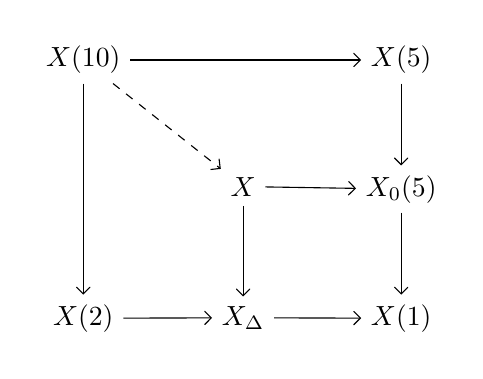
\begin{tikzpicture}[scale=2]
\matrix (m) [matrix of math nodes, row sep=3em, column sep=3em]
{ X(10) & & X(5)  \\
 & X & X_0(5)  \\
X(2) & X_{\Delta} & X(1)\\};
\path[->,font=\scriptsize,>=angle 90]
(m-1-1) edge  (m-3-1)
(m-1-1) edge (m-1-3)
(m-1-3) edge  (m-2-3)
(m-1-1) edge[dashed]  (m-2-2)
(m-2-3) edge  (m-3-3)
(m-2-2) edge  (m-2-3)
(m-2-2) edge  (m-3-2)
(m-3-1) edge  (m-3-2)
(m-3-2) edge  (m-3-3);
\end{tikzpicture}
\end{center}
where $X$ is the normalization of the fiber product $X_{\Delta} \times_{X(1)} X_0(5)$.  $X$ is an elliptic curve given by the equation
\[X: \qquad  y^2 = x^3 + 22x^2 +125x .\]
The map to $X_{\Delta}$ is given by
\[ (x,y) \mapsto \frac{y(x^2-500x -15625)}{x^3}. \]
Sage easily determines that $X$ is rank $0$, with rational points $(0:0:1)$ and $(0:1:0)$, both lying in the kernel of the map to $X_{\Delta}$.  \david{The target is $\P^1$ and doesn't have a kernel}. Thus our elliptic curve cannot give rise to a rational point on $X_0(5)$, and we conclude that $\rho_{E,5}$ is irreducible and thus absolutely irreducible.  \david{wait, this only gives irreducibility. What about absolutel irreducibility? You need to do the same construction for the normalizer of the nonsplit cartan. Ah, actually, your level is squarefree below, so it is absolutely irreducible.}
\end{proof}

\subsection{Proof of Theorem \ref{explicit_eg_thm}}

In this section we use the techniques of the modular method developed in the previous section to give a proof of our unconditional explicit theorem:

\begin{thm}\label{explicit_eg_thm_inplace}
For the following values of $b$ and $c$:
\begin{equation}\label{examples} (b,c) = (3,-2), (5,-6), (7,-12), (17,-72), (9,-20) \end{equation}
the Lucas sequence $u_n$ has no nontrivial $p$th powers, except $u_2 = 3^2$ in $(9,-20)$.
\end{thm}


If there exists a solution $u_n = y^p$ for $u_n$ in Theorem \ref{explicit_eg_thm_inplace} and $p \geq 5$, then by Lemma \ref{relprime} there exists a primitive solution to 
\[ X^p + 4(-c)^n Y^p = Z^p. \]
To this we associate the Frey curve of case 3 in Lemma \ref{freycurves}
\[E: Y^2 + XY = X^3 + \frac{w_n - 1}{4} X^2 + 2^{-4}(-c)^nX \]
The Frey curve $E$ has conductor and minimal discriminant
\[ N_E =\rad(c \cdot y)  \qquad \qquad \Delta_E = 2^{-8} \cdot (-c)^{2n} \cdot y^{2p}. \]
As $\Delta_E$ is a square, Lemma \ref{absirr} implies $\rho_{E,5}$ is absolutely irreducible.  In fact, this follows in general from the following lemma.

\begin{lem}\label{frey5irr}
Let $E$ be a Frey curve arising from a solution $u_n = y^5$ for $b^2+4c = 1$ and $n\geq 5$, then $\rho_{E,5}$ is absolutely irreducible.
\end{lem}
\begin{proof}
By Lemma \ref{freycurves} all of the discriminants of Frey curves of case (iii) are rational squares.  The result follows from Lemma \ref{absirr}.
\end{proof}

\begin{proof}[Proof of Theorem \ref{explicit_eg_thm}]
Posit a solution $u_n = y^p$ for $n \geq 7$ and $p \geq 5$.  To this solution, we associate a Frey curve $E$, as in the discussion above.  The mod $p$ Galois representation $\rho_{E,p}$ is unramified outside $p\cdot \rad{(c)}$ and finite flat at $p$ (except at $p=5$ in the last example) by Lemma \ref{unram}.   By Lemma \ref{absirr} and \ref{frey5irr} $\rho_{E,p}$ is absolutely irreducible for $p\geq 5$.  By the modularity of elliptic curves \ref{modularity} Ribet's level-lowering Theorem \ref{levellow}, the representation $\rho_{E,p}$ is isomorphic to one arising from a modular form of level $N = \rad(c)$.  For $b,c$ as above, there are no modular forms of level $\rad(c)=2,6,10$.  So there are no perfect $p$th powers if $p \geq 5$.

Invoking Lemma \ref{smallp} for the cases $p=2,3$ completes the proof of the theorem.
\end{proof}


\section{Proof of Theorem \ref{condbound}}\label{genthmproof}

In this section we give a proof of the following general theorem \textbf{conditional on the Frey-Mazur Conjecture}.  Let 
\[\psi(N) = N \cdot \prod_{p \mid N} \left( 1 + \frac{1}{p} \right) \]
be the Dedekind $\psi$ function.  Note that this is the index of $\Gamma_0(N)$ in the full modular group $\Gamma$. In addition 
\[ \dim S_2(\Gamma_0(N))_{\text{new}} \leq 1 + \frac{\psi(N)}{12} \]
for an exact formula see \cite{stein07}.

\begin{thm}\label{condbound_inplace}
Assume the Frey-Mazur conjecture.  Consider a solution (n,y,p) to \eqref{the_eqn}, with $n > 6$. Let $N = 2^8 \cdot \rad(c(b^2+4c))$. Then 
\[ p \leq \max\left\{17,   \psi(N)^{(\psi(N)/12 + 1)}, 3\log{|\alpha|} \cdot ( N+1)  \right\}. \]
\end{thm}

We break this into the following two theorems

\begin{thm}[]\label{bound_av}
Define ${\AV}(N)$ to be the maximum prime $p \in \Z$ such that there exists an elliptic curve $E/\Q$ which level lowers, mod $p$, to a modular abelian variety of level $N$, and dimension $> 1$.  Then
\[{\AV(N)} \leq \psi(N)^{(\psi(N)/12+1)}. \]
\end{thm}

\begin{thm}[]\label{bound_ell}
Let ${\Ell}(b,c)$ be the maximum prime $p \in \Z$ such that any Frey curve for the recurrence relation (b,c) level lowers, mod $p$, to an elliptic curve.  Assuming the Frey-Mazur Conjecture, 
\[{\Ell}(b,c) \leq \max\left\{17, 3\log{|\alpha|} \cdot (2^{8} \cdot \rad(c(b^2+4c))+1) \right\}. \]
\end{thm}


We spend the rest of this section proving these theorems. Theorem \ref{condbound} immediately follows.  Note that the bound for higher dimension abelian varieties is not conditional on the Frey-Mazur conjecture.



\subsection{Elliptic Curve Case and the Frey-Mazur Conjecture}

In the results that follow, we rely upon the following empirically-supported question of Mazur \cite{mazur78}, now referred to as the Frey-Mazur Conjecture, concerning the possibility of isomorphic Galois representations arising from non-isogenous elliptic curves.

\begin{conj}[Frey-Mazur]\label{FreyMazur}
Let $p > 17$, and $E_1$ and $E_2$ elliptic curves over $\Q$, with mod $p$ Galois representations $\rho_{E_1,p}$ and $\rho_{E_2,p}$ respectively.  If
\[ \rho_{E_1,p} \simeq \rho_{E_2,p} \]
then $E_1$ is isogenous to $E_2$.
\end{conj}

We prove our result \textbf{conditional on the Frey-Mazur Conjecture}. Our strategy is as follows: if the Frey curve $E$ corresponding to a solution $(n,y,p)$, $p > 17$, level lowers mod $p$ to an elliptic curve $F$, then the Frey-Mazur Conjecture implies that $N_E = N_F$. This forces $\rad(y)$ to divide the product of a fixed set of primes, depending only on $(b,c)$. Then, using general results on smooth numbers in recurrence sequences, we obtain a bound on $n$, in terms of $(b,c)$. We can then bound $p$ such that $y^p = u_n$ in terms of $n$.


\begin{thm}[\cite{gyory81}, \cite{gyory82}, \cite{gyory03}]\label{smoothterm}
Let $S$ be the set of all integers whose prime factors lie in some finite set $\{p_1,p_2,...,p_m\}$ with $p_m \geq p_i$ for all $i$.  Let $u_n$ be a Lucas sequence; for $n > 6$, if $u_n \in S$ then
\[ n \leq \max\{30, p_m +1 \}. \]
\end{thm}

\begin{lem}[Bound for $p$ in terms of $n$]\label{boundpintermsn}
For all solutions $u_n = y^p$, 
\[ p \leq 3n \log|\alpha|  \]
where $\alpha$ is the dominant root of the characteristic polynomial for $(b,c)$.
\end{lem}

\begin{proof}
It is clear that
\[p\log{2} \leq \log \bfrac{\alpha^n - \beta^n}{\alpha-\beta}  = \log|\alpha^{n-1}+ \alpha^{n-2}\beta+...+\beta^{n-1}|. \]
Thus as $|\alpha| \geq 2$
\begin{align*}
p & \leq  \frac{1}{\log{2}} \cdot \log|n\alpha^{n-1}| \\
%& \leq n \log_2|\alpha| +\log_2(n) \\
 & \leq 3\cdot n \log|\alpha|.
\end{align*}
\end{proof}

\begin{thm}\label{ell_bound_final}
Let $(b,c)$ relatively prime be a binary recurrence sequence with $u_0=0,u_1=1$. If $u_n = y^p$, and if the associated Frey curve level lowers mod p to an elliptic curve of level N, then assuming the Frey-Mazur conjecture, there exists an absolute, effectively computable constant $A_2$ such that
\[ p \leq \max\{17, \max\{30, 2^8 \cdot \rad(c(b^2+4c))+1\} \cdot A_2\log{\alpha} \}. \]
\end{thm}
\begin{proof}[Proof of Theorem \ref{bound_ell}]
Assume there exists a solution $u_n = y^p$, $n > 6$.
We associate a Frey curve $E$ to the Diophantine equation
\[ y^{2p} +4(-c)^n = v_n^2 \]
as in \ref{freycurves}.  By proposition \ref{freycurves}, the conductor of $E$ is
\[ N_E = 2^{\alpha}  \cdot \rad( c \cdot (b^2+4c) \cdot y) \qquad \qquad \alpha \leq 8. \]
By \ref{unram} the mod $p$ Galois representation $\rho_{E,p}$ is unramified outside $pN$, and flat at $p \notdiv c(b^2+4c)$. By assumption, there exists an elliptic curve $F$ such that
\[ \rho_{E,p} \simeq \rho_{F,p} \]  
with
\[N_F = 2^{\alpha} \cdot  \rad( c \cdot (b^2+4c)) \leq 2^8 \cdot \rad(c \cdot (b^2+4c))  \]
Invoking the Frey-Mazur conjecture \ref{FreyMazur}, $E$ and $F$ are isogenous, and thus $N_E = N_F$.  But these differ exactly in the primes dividing $y$, thus
\[ \rad(y) | \rad(2c \cdot (b^2+4c)). \]
 An application of \ref{smoothterm} and \ref{boundpintermsn} concludes the proof.
\end{proof}


\subsection{Higher Dimensional Abelian Variety Case}
We prove a general upper bound on the primes $p$ for which an irrational newform has mod $p$ Galois representation isomorphic to that of an elliptic curve.
 
Let $E$ be an elliptic curve and let $a_\ell$ denote the coefficients of the $L$-function of $E$.  If $\rho_{E,p} \simeq \bar{\rho_{f,p}}$ for $f$ a newform of level $N$ with Fourier coeffients $c_\ell\in \O_f$ for $K =  \Q(...,c_\ell,...)$ of degree $n_K = [K:\mathbb{Q}]$, then we have the following important lemma on necessary congruences.

\begin{lem}[\cite{cohen07}]\label{ircong1}
There exists a prime $\mathfrak{p} \mid p$ of $\mathcal{O}_f$ such that, for $\ell$ prime:
\begin{itemize}
\item $c_\ell \equiv a_\ell \mod \mathfrak{p}$, if $\ell \nmid pN$
\item $c_\ell^2 \equiv (\ell+1)^2 \mod \mathfrak{p}$, if $\ell \mid\mid N$
\end{itemize}
Further, as $|a_\ell| < 2\sqrt{\ell}$,
\[p \mid \gcd_{\ell^2 \nmid N}(B(\ell)C(\ell)), \] where
\[B(\ell) = \ell \cdot N_{K / \mathbb{Q}}(c_\ell^2-(\ell+1)^2) \]
\[C(\ell) = \prod_{-2\sqrt{\ell} < r < 2\sqrt{\ell}}{N_{K / \mathbb{Q}}}(c_\ell - r).\]
\end{lem}

For $n_K > 1$, this gives a nontrivial bound on $p$, as there exists an $\ell$ such that $c_\ell \notin \mathbb{Z}$ and $\ell^2 \nmid N$. For such an $\ell$, the product above is nonzero. We can bound $\ell$ using the following well-known theorem:
\begin{thm}[Sturm's Bound]\label{sturm}
Let $f,g \in M_k(\Gamma_0(N))$ have Fourier expansions $\sum_n a_nq^n$ and $\sum_n b_n q^n$ respectively.  Then $f = g$ if and only if $a_n = b_n$ for all
\[ n \leq \frac{k}{12} \cdot \psi(N). \]
\end{thm}

\begin{lem}\label{boundell}
Let $f$ be an irrational newform of level $N$.  If $\ell$ is the first prime such that $c_\ell \not\in \Z$, then
\[ \ell \leq (1/6) \cdot \psi(N) .\]
\end{lem}

\begin{proof}
Since $f$ has some irrational coefficient, we know there exists $\sigma \in G_\Q$, such that $f^{\sigma}$ is a distinct newform, also of level $N$.  Then, by \ref{sturm}, they must differ in an coefficient $c_\ell$ for some 
\[ \ell \leq \frac{1}{6} \psi(N). \]
\end{proof}

\begin{proof}[Proof of Theorem \ref{bound_av}]
Let $\ell$ be a prime such that $c_\ell \notin \Z$.  If $\ell^2 \mid N$, then $c_\ell = 0 \in \Z$, so we can assume $\ell^2 \notdiv N$. Thus we can apply Lemma \ref{ircong1}, 
\[ p \mid \ell \cdot N_{K / \mathbb{Q}}(c_\ell^2-(\ell+1)^2) \cdot \prod_{-2\sqrt{\ell} < r < 2\sqrt{\ell}}{N_{K / \mathbb{Q}}}(c_\ell - r).\]
It is clear that $|c_\ell^{\sigma}| < 2\sqrt{\ell}$ for all $\sigma \in \Gal(K/\Q)$. Thus, for $k \leq \ell+1$, \[N(c_\ell - k) \leq (\ell+1 + 2\sqrt{\ell})^{n_{K}}.\] 
By Lemma \ref{boundell}, we may take $\ell \leq (1/6)\psi(N)$, and $n_{K} \leq 1+\psi(N)/12$, thus
\[ p \leq \psi(N)^{(\psi(N)/12+1)}. \]
\end{proof}
 
 
 \begin{proof}[Proof of Theorem \ref{condbound}]
 Let $E$ be a Frey curve, such as in \ref{freycurves}.  Then if
 \[N_E = 2^\alpha {\rad}'(c(b^2+4c)y), \qquad \alpha \leq 8\]
where ${\rad}'$ denotes radical over odd primes, then $\rho_{E,p} \simeq \bar{\rho_{f,p}}$ for a newform $f$ of level
\[N_f =  2^\alpha {\rad}'(c(b^2+4c))\leq 2^8  {\rad}'(c(b^2+4c)) = N.\]
 If $f$ is irrational, we apply Theorem \ref{bound_av} to conclude that
 \[ p \leq \psi(N)^{(\psi(N)/12+1)}. \]
 If $f$ is rational, then we apply Theorem \ref{bound_ell} to conclude that
 \[ p \leq \max\left\{ 17, 3 \log|\alpha| \cdot (N+1) \right\}. \]
 The theorem easily follows.
 \end{proof}
 
\section{Examples}\label{examples}

As noted above, in many cases the conditional bounds achieved are in fact much better than the ``worst case" recorded in Theorem \ref{condbound}.  For any specific recurrence relation $(b,c)$, we can use the formulas for associating Frey curves in \ref{freycurves} to determine the possible levels to which the mod $p$ Galois representation descends, find all possible $p$ such that the representation arises from an irrational newform, and then invoke the Frey-Mazur conjecture to determine a bound on the index $n$ for which $u_n=y^p$ for any other $p \geq 17$.  

Given a reasonable bound on the index, it is trivial to check that there are no unknown perfect powers up to that index.  This leaves a finite list of primes $p$ for which there might exist a perfect $p$th power.  To deal with these primes, we develop a \textbf{completely elementary} sieve resembling that used in \cite{siksek06}, but not relying upon Frey curves.

\subsection{The Sieve}

Given a recurrence sequence $(b,c)$, fix $p$ a prime.  We want to find the complete list of solutions to $u_n = y^p$.  Let $q \equiv 1 \pmod{p}$ be a prime.  Define $K(q)$ to be the period of the Fibonacci sequence mod $q$.  As $p$ necessarily divides the order of $\F_q^\times$, there should be only $1/p$ perfect $p$th powers in our sequence modulo $q$.  

Construct a set $\N(q) \subseteq \Z/K(q)\Z $ consisting of possible values of the index $n \mod{K(q)}$ such that $u_n$ is perfect $p$th power mod $q$.  For any set $S = (q_1,q_2,...,q_m)$, denote $K(S) = \lcm(K(q_1),...,K(q_m))$ and $\N(S)$ the ``intersection" of the sets $K(q_1)$ coming from the Chinese Remainder Theorem.


As in \cite{siksek06}, we choose $q_i$ such that $K(q_i)$ are all particularly smooth, ie such that 
\[K(S) \mid M = 2^5 \cdot 3^3 \cdot 5^2 \cdot 7 \cdot 11.\]
With enough primes $q_i$, we will get a small number of congruences modulo a large modulus.  Once $K(S) = M$, we replace $M$ by $M  \cdot 13$ and continue again. 

The congruences $n \equiv 0,1 \pmod{K(S)}$ will always be present in $\N(S)$ as they are $p$th powers for any $p$.  In addition, if there exists another nontrivial $p$th power, this will appear as an added congruence in $\N(S)$ that does not grow with the modulus.  However, if in fact these are the only $p$th powers, then any remaining elements of $\N(S)$ should grow with the modulus $M$.  

Coming from Thue equations and linear forms in logarithms, **we hope to have a bound**  $B(n,p)$ for $n$ in terms of $p$.  If there are no other elements of $\N(S)$ that grow with $M$, then once $M >B(n,p)$, we have found all of the perfect powers.  If there are elements that grow with $M$, then once the smallest $\bar{a} \in \N(S)$ is large enough such that $\bar{a} > B(n,p)$, we have found all perfect $p$th powers.






%\subsection{Proof of Theorem \ref{cond_ex}}

%***we think we might be able to prove this theorem.  At the moment we can bound $p \leq 19$ in all of %these cases, and are running the sieve to find a lower bound on n, but we still need an upper bound %from Thue equations/lin forms in logs which might be hard***


%\begin{thm}\label{cond_ex_inplace}
%Assume the Frey-Mazur Conjecture.  For $(b,c)$ a nondegenerate Lucas sequence with $1 \leq b,c \leq %10$ relative prime, the only perfect powers besides $u_0=0,u_1=1$, and $u_2 = b$ (in the cases $b$ is %a perfect power) are:
%\begin{center}
%\begin{tabular}{c | c || c | c}
%$\mathbf{(b,c)}$ & $\mathbf{u_n=y^p}$ & $\mathbf{(b,c)}$ & $\mathbf{u_n = y^p}$ \\ \hline
%$(1,1)$ & $u_6 = 2^3, u_{12} = 12^2$ & $(2,7)$ & $u_4 = 6^2$ \\
%$(1,3)$ & $u_3 = 2^2$ & $(3,7)$ & $u_3 = 2^4$ \\
%$(1,4)$ & $u_4 = 3^2, u_8 = 21^2$ & $(3,8)$ & $u_5 = 19^2$ \\
%$(1,7)$ & $u_3 = 2^3$ & $(4,9)$ & $u_3 = 5^2$ \\
%$(1,8)$ & $u_6 = 15^2$ & $(5,2)$ & $u_3 = 3^3$ \\
%$(2,1)$ &  $u_7 = 13^2$ & $(5,7)$ & $u_3 = 2^5$ \\
%$(2,5)$ & $u_3 = 3^2$ \\
%\end{tabular}
%\end{center}
%\end{thm}







\bibliography{bib}{}
\bibliographystyle{amsalpha}


\end{document}